% This is samplepaper.tex, a sample chapter demonstrating the
% LLNCS macro package for Springer Computer Science proceedings;
% Version 2.20 of 2017/10/04
%
\documentclass[runningheads]{llncs}
%
%
\usepackage{graphicx}
% Used for displaying a sample figure. If possible, figure files should
% be included in EPS format.
%
% If you use the hyperref package, please uncomment the following line
% to display URLs in blue roman font according to Springer's eBook style:
% \renewcommand\UrlFont{\color{blue}\rmfamily}

\begin{document}
%
\title{A novel distributed nature-inspired algorithm for solving optimization problems\thanks{Supported by organization x.}}
% (Biological) Life-Cycle Algorithm: A novel distributed nature-inspired algorithm for solving optimization problems
%
%\titlerunning{Abbreviated paper title}
% If the paper title is too long for the running head, you can set
% an abbreviated paper title here
%
\author{First Author\inst{1}\orcidID{0000-1111-2222-3333} \and
Second Author\inst{2,3}\orcidID{1111-2222-3333-4444} \and
Third Author\inst{3}\orcidID{2222--3333-4444-5555}}
%
\authorrunning{F. Author et al.}
% First names are abbreviated in the running head.
% If there are more than two authors, 'et al.' is used.
%
\institute{Princeton University, Princeton NJ 08544, USA \and
Springer Heidelberg, Tiergartenstr. 17, 69121 Heidelberg, Germany
\email{lncs@springer.com}\\
\url{http://www.springer.com/gp/computer-science/lncs} \and
ABC Institute, Rupert-Karls-University Heidelberg, Heidelberg, Germany\\
\email{\{abc,lncs\}@uni-heidelberg.de}}
%
\maketitle              % typeset the header of the contribution
%
\begin{abstract}
%The abstract should briefly summarize the contents of the paper in 150--250 words.

Several bio-inspired algorithms use population evolution as analogies of
nature. In this paper, we present an algorithm inspired by the biological
life-cycle of animal species, which consists of several stages: birth, growth,
reproduction, and death. As in nature, we intend to execute all these stages in
parallel and asynchronously on a population that evolves constantly. From the
ground up, we designed the algorithm as a cloud-native solution using the cloud
available resources to divide the processing workload, among several computers
or running the algorithm as a cloud service. The algorithm works concurrently
and asynchronously on a constantly evolving population, using different
computers (or containers) independently, eliminating waiting times between
processes. This algorithm seeks to imitate the natural life cycle, where new
individuals are born at any moment and mature over time, where they age and
suffer mutations throughout their lives. In reproduction, couples match by
mutual attraction, where they may have offspring. Death can happen to everyone:
from a newborn to an aged adult, where the individual's fitness will impact
their longevity. As a proof-of-concept, we implemented the algorithm with
Docker containers by solving the OneMax problem comparing it with a basic
(sequential) GA algorithm, where it showed favorable and promising results.

\keywords{First keyword  \and Second keyword \and Another keyword.}
\end{abstract}

\section{Introduction} 

Bio-inspired algorithms have been very successful when
used to solve complex optimization problems, but as their complexity increases
so does the computing power required. One strategy to address this processing
need is to use distributed computing, or the resources available in the cloud
to help find the solution. This strategy gives us elasticity to increase (or
reduce) the computing power to achieve a balance according to the nature of the
problem.

One of the problems that we have identified in this research is that most
bio-inspired algorithms are designed with a traditionally sequential
perspective, where each process must wait for the previous task to finish
before continuing. Some architectures address this issue, what distinguishes
us, is that our proposal presents an algorithm designed in its entirety as a
native solution in the cloud, fully distributed, where its processes are
executed in parallel and asynchronously. This technique makes it easy to scale
the computing power according to the complexity required by the problem.

We designed our algorithm using observation, analysis, and abstraction in
nature to identify what most species in the animal kingdom have in common,
where individuals of a population that best adapt to the environment have
greater chances of survival, reproduction, and improvement of the species.
Imagining as if the task of writing these rules of evolution was in our hands,
questioning how we could solve it?

Similar to nature, we identified what most species have in common in the life
cycle. Our algorithm works on a constantly evolving population, experiencing
the stages that all living beings undergo: being born, growing up, reproducing,
and dying, where each of these stages will be processes (of our algorithm) that
randomly affect the population individuals, emulating the organic way.

This algorithm seeks to imitate the natural life cycle, where new individuals
are born at any moment and mature over time, where they age and suffer
mutations throughout their lives. In reproduction, couples match by mutual
attraction, where they may have offspring. Death can happen to everyone: from a
newborn to an aged adult, where the individual's fitness will impact their
longevity.

In this research, we seek to demonstrate that it is possible to evolve a
population of individuals, similar to a Genetic Algorithm (GA), using a
distributed, parallel, and asynchronous methodology.


\section{Description of the sections of the Paper} 

\section{State of the art} 

One of the publications with the most influence and impact on our research,
which inspired us to carry out this project is "A container-based cloud-native
architecture for the reproducible execution of multi-population optimization
algorithms" by Mario García Valdez and Juan J. Merelo Guervós.

They propose a cloud-native optimization framework, that can include multiple
(population-based) algorithms without increasing the number of parameters that
need tuning. Their solution can support different algorithms at the same time,
work asynchronously, and also be readily deployable to any cloud platform.

"Splitting a population into multiple instances is a technique used extensively
in recent years to help improve the performance of nature-inspired optimization
algorithms. Work on those populations can be done in parallel, and they can
interact asynchronously, a fact that can be leveraged to create scalable
implementations based on, among other methods, distributed, multi-threaded,
parallel, and cloud-native computing". [All of the above taken from their publication]

[Note: This draft is a work in progress, needs improvement]


\section{Proposal} 

From the ground up, we designed the algorithm as a cloud-native solution using
the cloud available resources to divide the processing workload, among several
computers or running the algorithm as a cloud service. The algorithm works
concurrently and asynchronously on a constantly evolving population, using
different computers (or containers) independently, eliminating waiting times
between processes.

In this paper, we present an algorithm inspired by the biological life-cycle of
animal species, which consists of several stages: birth, growth, reproduction,
and death. As in nature, we intend to execute all these stages in parallel and
asynchronously on a population that evolves constantly. This algorithm starts
with a randomly generated population, where the processes will interact with
the population independently. This means that at any given time, any individual
can experience any of these processes.


\subsection{Birth}

Similar to a GA, our algorithm starts with the process responsible for the
random generation of individuals. In our scheme, we call it birth, however, we
must mention that the successful reproduction process will result in the birth
of new individuals (offspring).

\subsection{Growth}

As in nature, all individuals constantly grow, mature, or age. With increasing
age, individuals may lose strength but also gain more knowledge to solve
problems. We represent this with a possible mutation in each increment of age.
The growth process will take an individual to assess whether it's ready to
mature and undergo changes.

\subsection{Reproduction}

The attraction of a couple will depend on fitness: the better individual's
fitness, the more attractive it will be, making it easier to find mating
matches. Not all couples will be compatible, so reproduction will not always be
possible, but the problem arises: how to quantify the attraction between two
individuals?. The reproduction process will be taking random pairs of
individuals to evaluate their attraction as a couple, to try to breed; when the
gestation is successful, a new pair of individuals will be born (as the
offspring).

\subsection{Death}

The process of dying represents the challenges and adversities that life
presents (to overcome). This process evaluates the individual resistance to
survive in the environment. The better fitness the individual has will increase
its chances of survival. As time progresses, the demands of nature will also
increase, pushing for only the best individuals to survive.


\section{Experimental} 

As a proof-of-concept, we implemented the algorithm with Docker containers by
solving the OneMax problem comparing it with a basic (sequential) GA algorithm,
where it showed favorable and promising results.

%
%
%

% Introducción 
% Contexto: Los algoritmos bioinsirados se utilzan para resolver 
% problemas complejos, pero en ocasiones se requiere de poder
% computo.
% Problemas: La mayoría de los algoritmos bio inspiarados
% no están diseñandos con perspectiva distribuida, paralela y asíncrona. 
% De que hay arquitecturas que tratan esta problematica. 
% Propuesta. 
% Descripción de las secciones del paper.

% Estado del Arte 
% PSO distribuido, GAs, etc.

% Propuesta
% 

% Experimental 
% Setup 
% OneMax
% Results 

% Conclusiones

\section{Another Section}
\subsection{A Subsection Sample}
Please note that the first paragraph of a section or subsection is
not indented. The first paragraph that follows a table, figure,
equation etc. does not need an indent, either.

Subsequent paragraphs, however, are indented.

\subsubsection{Sample Heading (Third Level)} Only two levels of
headings should be numbered. Lower level headings remain unnumbered;
they are formatted as run-in headings.

\paragraph{Sample Heading (Fourth Level)}
The contribution should contain no more than four levels of
headings. Table~\ref{tab1} gives a summary of all heading levels.

\begin{table}
\caption{Table captions should be placed above the
tables.}\label{tab1}
\begin{tabular}{|l|l|l|}
\hline
Heading level &  Example & Font size and style\\
\hline
Title (centered) &  {\Large\bfseries Lecture Notes} & 14 point, bold\\
1st-level heading &  {\large\bfseries 1 Introduction} & 12 point, bold\\
2nd-level heading & {\bfseries 2.1 Printing Area} & 10 point, bold\\
3rd-level heading & {\bfseries Run-in Heading in Bold.} Text follows & 10 point, bold\\
4th-level heading & {\itshape Lowest Level Heading.} Text follows & 10 point, italic\\
\hline
\end{tabular}
\end{table}


\noindent Displayed equations are centered and set on a separate
line.
\begin{equation}
x + y = z
\end{equation}
Please try to avoid rasterized images for line-art diagrams and
schemas. Whenever possible, use vector graphics instead (see
Fig.~\ref{fig1}).

\begin{figure}
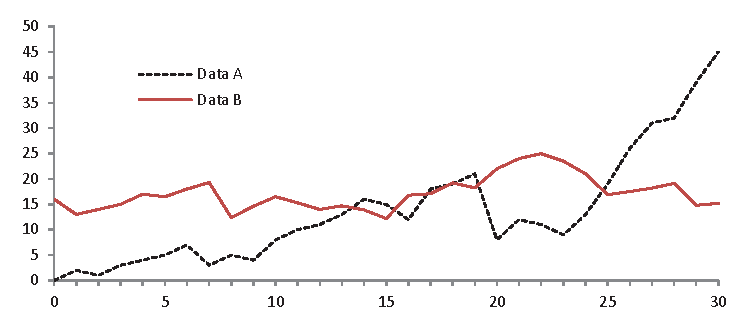
\includegraphics[width=\textwidth]{fig1.eps}
\caption{A figure caption is always placed below the illustration.
Please note that short captions are centered, while long ones are
justified by the macro package automatically.} \label{fig1}
\end{figure}

\begin{theorem}
This is a sample theorem. The run-in heading is set in bold, while
the following text appears in italics. Definitions, lemmas,
propositions, and corollaries are styled the same way.
\end{theorem}
%
% the environments 'definition', 'lemma', 'proposition', 'corollary',
% 'remark', and 'example' are defined in the LLNCS documentclass as well.
%
\begin{proof}
Proofs, examples, and remarks have the initial word in italics,
while the following text appears in normal font.
\end{proof}
For citations of references, we prefer the use of square brackets
and consecutive numbers. Citations using labels or the author/year
convention are also acceptable. The following bibliography provides
a sample reference list with entries for journal
articles~\cite{ref_article1}, an LNCS chapter~\cite{ref_lncs1}, a
book~\cite{ref_book1}, proceedings without editors~\cite{ref_proc1},
and a homepage~\cite{ref_url1}. Multiple citations are grouped
\cite{ref_article1,ref_lncs1,ref_book1},
\cite{ref_article1,ref_book1,ref_proc1,ref_url1}.
%
% ---- Bibliography ----
%
% BibTeX users should specify bibliography style 'splncs04'.
% References will then be sorted and formatted in the correct style.
%
\bibliographystyle{splncs04}
\bibliography{bib/bibliografia.bib}
%
\end{document}
